\documentclass{article}
\usepackage{color}
\usepackage[english]{babel}
\renewcommand{\figurename}{Figur}
\usepackage[utf8]{inputenc}
\usepackage[T1]{fontenc}
\usepackage{amssymb}
\usepackage{amsmath}
\usepackage{mathtools}
\usepackage{commath}
\usepackage{lmodern}
\usepackage{units}
\usepackage{icomma}
\usepackage{color}
\usepackage{graphicx}
\usepackage{float}
\usepackage{caption}
\usepackage{subfiles} % Paket för att inkludera TeX-filer
\setlength{\parindent}{0pt}
\setlength{\parskip}{12pt}
\setlength{\intextsep}{0pt plus 2pt}



\begin{document}
\title{Title}
\author{Olof Sjödin \thanks{olsj@kth.se} \and Sven Svensson
\thanks{sven@svensson.com}}
\date{4 June 2015}
\maketitle

\vspace*{18\baselineskip}
\begin{center}
    Sample Course - SI1337\\
    Royal Institute of Technology
\end{center}
\thispagestyle{empty}
\newpage

\section{Introduction}
Bla bla bla.

\section{Theory}
Bla bla bla.

\section{Results}


Our final result of the fit is shown in figure \ref{fig:curvefit}.

\begin{figure}[H]
\centering
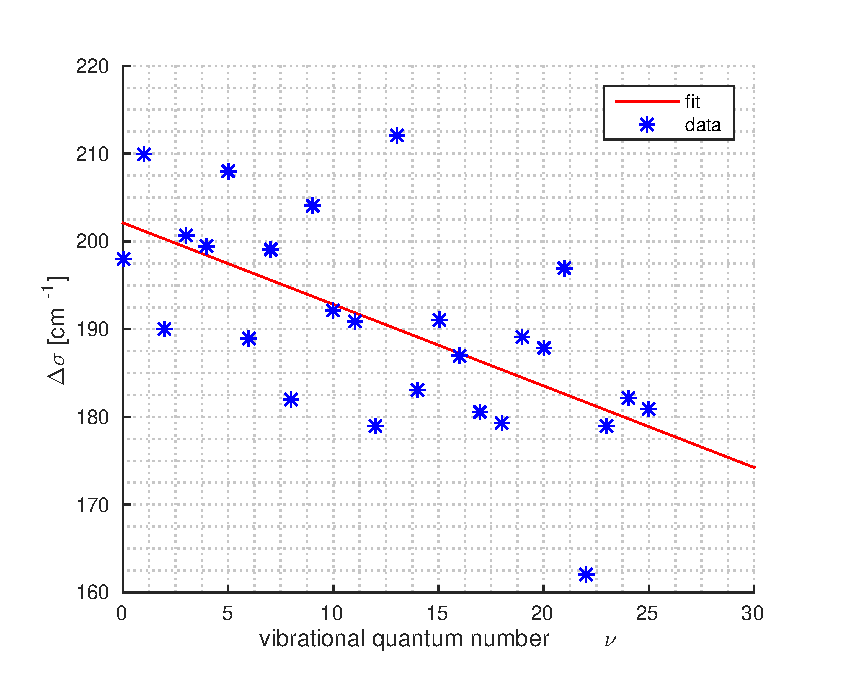
\includegraphics{fit-including-missing-peaks.eps}
\caption{Fitting the data to the to the linear equation $\Delta \sigma = \omega_e-2\omega_ex_e(1+\nu)$ with inserted peaks. $R^2=0.3828$}
\label{fig:curvefit}
\end{figure}

$\omega_e= 214.50 cm^{-1}$ and $\omega_ex_e = 0.614 cm^{-1}$ was retrieved 
from NiST\cite{2} is the reference value or theoretical value.
The result we got from the last fit is $\omega_e 202.5803^{-1}$ which is a $5.557\%$ deviation from the theoretical value, $\omega_ex_e=0.46463cm^{-1}$ which is a $24.3277\%$ deviation and $D_e=22081.5347cm^{-1}$ that is a $17.8751\%$ deviation. 

You can see the peaks that are used in figure \ref{fig:curvefit} at table \ref{tabell}.

\vspace{5mm}
    \begin{table}[H]
        \captionsetup{width=0.85\textwidth}
        \centering
        \begin{tabular}{| l | l |}
            \hline
            Vibrational quantum number $\nu$    & $\Delta\sigma$ [$10^4 cm^{-1}$] \\ \hline
            4                    & 1.8828                 \\ \hline
            11                   & 1.7455                 \\ \hline
            18                   & 1.6131                 \\ \hline
            20                   & 1.5763                 \\ \hline
            25                   & 1.4855                 \\ \hline
        \end{tabular}
        \caption{Inserted peaks that are used in figure \ref{fig:curvefit}}
        \label{tabell}
    \end{table}

\section{Discussion}


\begin{thebibliography}{1}
\bibitem{1} ChemeDDL.org \texttt{http://www.chemeddl.org/alfresco/service/api/node/content/workspace/\\SpacesStore/8a367d14-7f6d-4fef-a7df-eb19579da11b/IodineSpectrum.pdf?guest=true}
\bibitem{2} NiST
\texttt{http://webbook.nist.gov/cgi/cbook.cgi?ID=C7553562\&Units=SI\&Mask=1000}

\end{thebibliography}

\end{document}
